\chapter{Thuật toán PODEM}
\label{sec:p3-podem}
% Bản ngắn theo README/kế hoạch P1; chi tiết trong notes/p3_*.
\textbf{Nguyên lý.}
PODEM (Goel, 1981) chỉ ra quyết định nhị phân tại PI; các net nội bộ
được suy ra bằng mô phỏng, nên không cần J-frontier như D-algorithm
\cite{p3_goel1981,p1_wang2006}. Cây tìm kiếm trên $n$ PI có tối đa $2^n$
vector đầy đủ; trường hợp xấu vẫn cần tìm kiếm theo hàm mũ.
\emph{Objective} chọn $(l,1-s)$ để kích hoạt lỗi $l/\mathrm{SA}s$;
sau kích hoạt, chọn đầu vào X của D-frontier về giá trị không điều khiển
(1 cho AND/NAND, 0 cho OR/NOR).
\emph{Backtrace} đưa mục tiêu về PI chưa gán, đảo bit qua NAND/NOR/NOT;
\emph{imply} tính lại toàn mạch bằng logic $0,1,X,D,D'$.
P3-v1 chọn cổng theo topo ổn định và đầu vào X đầu tiên trong netlist,
không dùng SCOAP.

\textbf{Bổ sung XOR/XNOR (P3-v1.1).}
\label{sec:p3-xor-xnor}
Đặt $y=x_1\oplus\cdots\oplus x_n\oplus q$, với $q=0$ cho XOR,
$q=1$ cho XNOR. Backtrace mục tiêu $y=v$: nếu chỉ còn một đầu vào X,
giá trị cần tại đó là $v\oplus q\oplus p$, trong đó $p$ là parity
các bit mạch tốt đã biết ($D\mapsto1$, $D'\mapsto0$).
Nếu còn nhiều X, chọn X đầu tiên và thử 0, imply rồi tính lại.
Objective lan truyền cũng ưu tiên X đầu tiên bằng 0; XOR/XNOR không có
giá trị điều khiển. Ví dụ $D\oplus0=D$, $D\oplus1=D'$,
nhưng $D\oplus D=0$: nhiều nhánh lỗi có thể triệt tiêu.
XNOR đảo kết quả XOR đúng một lần. Quy tắc, bảng và ví dụ chi tiết ở
\nolinkurl{notes/p3_xor_xnor.md}; đặc tả này đã được P5 triển khai và kiểm thử trong bản tích hợp.

\textbf{Dừng và quay lui.}
Có $D/D'$ ở PO thì thành công. Khi lỗi đã kích hoạt nhưng không
còn đường X từ D-frontier tới PO, nhánh thất bại; có X-path chỉ là điều kiện
cần. Frontier rỗng trước kích hoạt chưa đủ để loại nhánh.
Mã giả: \emph{imply $\to$ kiểm tra PO/khả thi $\to$ objective/backtrace
$\to$ thử PI $b$ $\to$ nếu thất bại, kiểm tra giới hạn rồi thử $1-b$
$\to$ nếu cả hai thất bại, trả PI về X và quay về cha}.
Xóa quyết định con trước khi đảo cha. Đếm backtrack bằng số phép đảo PI;
hết cây mới kết luận UNTESTABLE, hết giới hạn là ABORTED.
Lưu đồ và cây đầy đủ ở \nolinkurl{report/figures/p3/}; giải thích trong
\nolinkurl{notes/p3_ly_thuyet.md}.

\textbf{c17, lỗi stem $11/\mathrm{SA0}$.}
Theo PI $(1,2,3,6,7)$, P3-v1 cho Bảng~\ref{tab:p3-c17}.

\begin{table}[htbp]\centering\small
\caption{Hai phép gán PI; các net chưa liệt kê giữ X.}
\label{tab:p3-c17}
\begin{tabular}{@{}clll@{}}\toprule
Bước & Objective; PI & Net xác định sau imply & D-frontier\\\midrule
1 & $(11,1)$; $3=0$ & $10=1,11=D$ & $\{16,19\}$\\
2 & $(2,1)$; $2=1$ & $10=1,11=D,16=D',22=D$ & $\{19,23\}$\\\bottomrule
\end{tabular}
\end{table}

Vì $3=0$ nên NAND11 tốt bằng 1; $2=1$ truyền $D$ qua NAND16 thành
$D'$, rồi qua NAND22 thành $D$. Pattern $X10XX$, 0 backtrack;
8/8 cách điền X phát hiện lỗi tại 22. Điền X=0 được $01000$,
PO tốt $(1,1)$, lỗi $(0,0)$. PO23 còn X trong trace là xấp xỉ bảo thủ.

% P2 bb3756d: common/c17.tex chỉ chứa includegraphics, không phải float.
\begin{figure}[htbp]\centering
\begin{minipage}{0.49\linewidth}\centering
\IfFileExists{figures/common/c17.tex}{\resizebox{\linewidth}{!}{% P2: tái sử dụng hình mach_c17.jpg do người dùng cung cấp, không vẽ lại.
% Wrapper dùng được từ report/main.tex và slides/main.tex.
% Hình thể hiện cube tổng quát hóa (X,1,0,X,X).
\IfFileExists{figures/common/mach_c17.jpg}{%
  \includegraphics[width=0.72\linewidth]{figures/common/mach_c17.jpg}%
}{%
  \includegraphics[width=0.72\linewidth]{../report/figures/common/mach_c17.jpg}%
}
}}{%
\resizebox{\linewidth}{!}{% Sơ đồ liên kết tín hiệu, mọi khối đều là NAND. Dùng tạm khi chưa có hình P2.
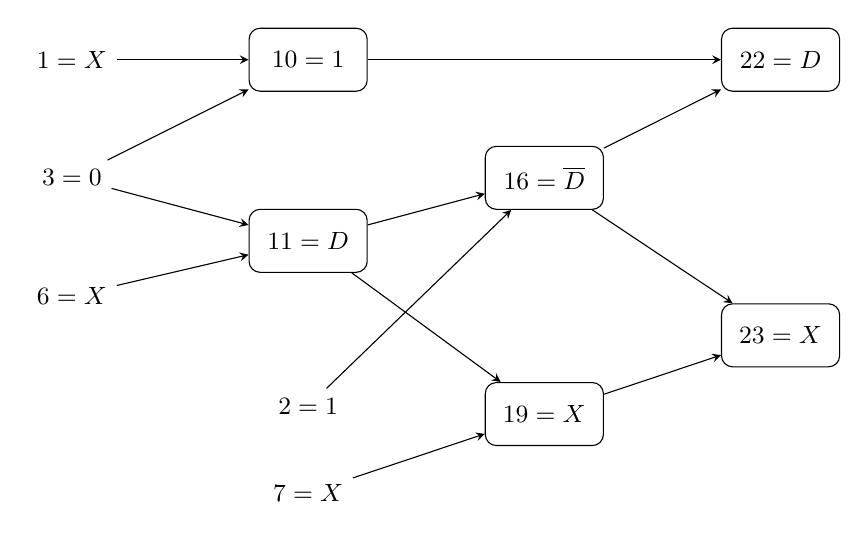
\begin{tikzpicture}[x=1cm,y=1cm,every node/.style={font=\small},gate/.style={draw,rounded corners,minimum width=1.5cm,minimum height=0.8cm,align=center},>=stealth]
\node (i1) at (0,3) {$1=X$}; \node (i3) at (0,1.5) {$3=0$};
\node (i6) at (0,0) {$6=X$}; \node (i2) at (3,-1.4) {$2=1$};
\node (i7) at (3,-2.5) {$7=X$};
\node[gate] (g10) at (3,3) {$10=1$};
\node[gate] (g11) at (3,0.7) {$11=D$};
\node[gate] (g16) at (6,1.5) {$16=\overline D$};
\node[gate] (g19) at (6,-1.5) {$19=X$};
\node[gate] (g22) at (9,3) {$22=D$};
\node[gate] (g23) at (9,-0.5) {$23=X$};
\draw[->] (i1)--(g10); \draw[->] (i3)--(g10); \draw[->] (i3)--(g11); \draw[->] (i6)--(g11);
\draw[->] (g11)--(g16);\draw[->] (g11)--(g19);\draw[->] (i2)--(g16);\draw[->] (i7)--(g19);
\draw[->] (g10)--(g22);\draw[->] (g16)--(g22);\draw[->] (g16)--(g23);\draw[->] (g19)--(g23);
\end{tikzpicture}
}}
\end{minipage}\hfill
\begin{minipage}{0.49\linewidth}\centering
\resizebox{\linewidth}{!}{\begin{tikzpicture}[every node/.style={font=\small,align=center},level distance=1.6cm,sibling distance=5.8cm]
\node[draw,rounded corners] {Objective $t=1$\\Chọn PI $a$}
 child {node[draw] {$a=1$: $t=D$, $n=0$\\$out=0$: nhánh thất bại}
 edge from parent node[left] {thử trước}}
 child {node[draw] {$a=0$: $t=X$, $n=1$}
 child {node[draw,rounded corners] {$b=1$: $out=D$\\DETECTED, vector $01$}
 edge from parent node[right] {objective $t=1$}}
 edge from parent node[right] {đảo 1 lần}};
\end{tikzpicture}
}
\end{minipage}
\caption{Trái: c17 ở trạng thái cuối (hình P2 nếu có;
dự phòng P3: mọi khối là NAND).
Phải: cây quyết định mạch phụ, thử $a=1$ rồi đảo $a=0$.}
\label{fig:p3-examples}
\end{figure}

\textbf{Ví dụ quay lui.}
Mạch phụ $t=a+b$, $n=\overline a$, $out=tn$, lỗi stem $t/\mathrm{SA0}$:
thử $a=1$ cho $(t,n,out)=(D,0,0)$, nhánh thất bại với mọi $b$;
đảo $a=0$ cho $(X,1,X)$; chọn lại objective $(t,1)$, gán $b=1$
cho $(D,1,D)$. Kết quả $01$, ba hàng gán/đảo, một backtrack.
Giới hạn 0 phải ABORTED trước phép đảo, không phải UNTESTABLE.
Hai trace đủ bảy cột ở \nolinkurl{results/golden_trace_c17_11sa0.md}
và \nolinkurl{results/golden_trace_backtrack.md}.

\textbf{So sánh và đối chiếu nhóm.}
Trace tay P2 trên nhánh \nolinkurl{p2-d-algorithm} có 4 lần chọn cube
(không đếm implication), 3 PI được gán, 0 backtrack, pattern $X100X$;
sau tổng quát hóa được $X10XX$. P3 có 2 phép gán PI, 0 backtrack.
Hai đơn vị đếm khác nhau, không suy ra tỷ lệ tăng tốc.
D-algorithm cần justification các quyết định nội bộ; PODEM dùng backtrace
và imply. FAN cải tiến lựa chọn bằng cấu trúc fanout và multiple backtrace
\cite{p3_fujiwara1983}; nhóm chưa cài FAN.
Bộ kiểm chứng P3 duyệt 32 vector c17, 4 vector mạch phụ và 22 lỗi stem;
đạt các kỳ vọng trên. Bộ kiểm thử tích hợp đã đối chiếu trace P5 đủ bảy
cột, hai phép gán PI trên c17 và một backtrack trên mạch phụ;
simulator P6 xác nhận cả hai mẫu.
Nguồn P2, khác biệt heuristic và danh sách đầu vào thiếu ở
\nolinkurl{notes/p3_doi_chieu_P5.md}.
